\documentclass[12pt]{article}

\usepackage[margin=1in]{geometry}

\usepackage{times}

\usepackage{hyperref}
\hypersetup{
    colorlinks=true,
    linkcolor=blue,
    filecolor=magenta,      
    urlcolor=blue,
}
 
\urlstyle{same}

\usepackage{datetime}
\newdateformat{specialdate}{\twodigit{\THEDAY}.\twodigit{\THEMONTH}.\THEYEAR}

\usepackage[utf8]{inputenc}

\usepackage{titling}

\usepackage{framed}
\usepackage[svgnames]{xcolor}
\colorlet{shadecolor}{Gainsboro!50}

\usepackage{float}
\usepackage{graphicx}
\graphicspath{ {./images/} }

\usepackage{verbatim}

\usepackage{caption}
\captionsetup[figure]{name=Fig.}

\begin{document}
\begin{center}
\textbf{Benchmarking of sequence preprocessing step for the family classification task}
\end{center}


\begin{center}
Sikora Maciej$^{1}$
\end{center}

[1] Faculty of Mathematics, Informatics and Mechanics, University of Warsaw, Poland \newline

\section*{Abstract}
With the growing amount of protein data, there is a need for improving automated prediction models. However, more sophisticated ones are increasingly resource-heavy and slower, thus requiring preprocessing steps to yield satisfying results in finite time. Because successful compression of biological sequences should speed up the learning process without losing crucial information, standard string compression might not fit here. Instead, protein-dedicated models are required, taking advantage of the smaller amino acid alphabet as well as factoring wider biological context behind one-letter abbreviations.
Context analysing and learning models aren't a specific to protein data and are commonly used in natural language text analysis. Multiple such preprocessing models can be formulated as well as multiple algorithms can be used for the learning process depending on the research goal. Here we show a step-by-step comparison between several preprocessed protein datasets for the family classification tasks, evaluating with most common multi-class classifier algorithms with runtime and accuracy as metrics. Results show how important the sequence preparation step is, significantly improving model quality. We also highlight, that in pursuit of size reduction we shouldn't forget about accuracy assessment.

\section*{Introduction}
For the last 5 years unannotated part of the Uniprot database -- Swissprot, increased over 3 times from 73,711,881 (release 2017\_01) to 230,328,648 entries (2022\_01) [1]. If the trend continues, such an enormous amount of data will be challenging to process outside the large servers and supercomputers. Such a prospect inspires many scientists to look closely into data preprocessing to speed up the research. However, naive data reduction might not necessarily be the best solution, when increased speed is connected with loss of information. Our goal for the project is to provide a modular workflow testing multiple data preprocessing techniques and commonly used data classification models. We are going to compare the size of the files and speed, but also the accuracy of the models to answer questions like what is the best protein sequential data preprocessing method? Is such a method universal to all the research problems? What can we do to improve our results further? What might be the future of data preprocessing?

\section*{Methods and materials}
\begin{figure}[H]
\begin{center}
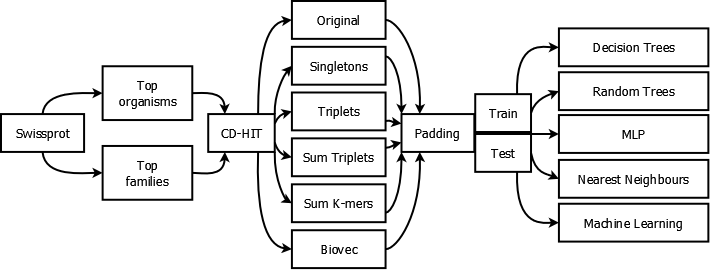
\includegraphics[width=0.9\textwidth]{workflow}
\caption{Diagram of the workflow of the project. Shows the following steps of preprocessing and evaluation. Its modular structure allows for potential further extensions in every section.}
\end{center}
\end{figure}

\subsubsection*{Data preparation}
In the article we will use all SwissProt entries as a base for the Pfam[2] family classification problem. Such a choice is fundamental for two reasons. Data is already annotated, thus possible to evaluate after the learning process. SwissProt entries are also manually verified, so the dataset should contain less noise - providing a much cleaner environment for testing.

Before encoding our data, however, some universal preprocessing steps are required. First, only entries with a single domain are chosen for further analysis. While multi-domain sequences are possible to evaluate using one-hot encoding, they are often much longer and more complex with additional linkers. 
Even further, sequences of length below 50 and above 2000 are filtered out. Both steps can be treated as discarding outliers, and are especially important for the padding step mentioned later. 

At this point, however, a dataset is still too big to be fed into our models. To reduce the size, only a selection of organisms and Pfam families will be used. In this project, we suggested the 10 largest families and 2000 most frequent organisms (Precise data can be verified and tweaked in the source code provided). 

Another step addresses very similar proteins. This workflow uses CD-HIT[3] as a tool of choice. This package is designed to cluster sequences above a certain threshold of sequential similarity and pick only one exemplar, effectively thinning out our dataset from duplicates. In this project, we used non-invasive filtering with 99\% similarity. 

For further evaluation dataset was divided into training and test sections. There are 7900 training sequences (790 per family) and 1050 testing ones (105 per family). Those numbers were picked arbitrally and scaled to the family with the lowest number of representatives.

\subsubsection*{Data models}
\begin{figure}[H]
\begin{center}

\includegraphics[width=0.7\textwidth]{vec}
\caption{Summary of data models. This project compares six representations: original, singletons, triplets, sum triplets, sum k-mers and BioVec.}
\end{center}
\end{figure}

In this project, we were testing 6 data models. They will present a step-by-step progression from original data to more complex encoding. For each model, there will be discussed the idea behind it, its advantages and limitations and how it might affect the data. Preprocessing methods can be divided into two categories: ''In-place'' and ''restructuring''. In-place methods are reforming the way sequence is presented to training models by changing the representation and data type. Restructuring models deviate from this rule, only extracting information from the dataset and forming feature vectors. While restructuring models and Biovec already produce vectors of the same length, in-place methods require sequences to be manually padded to the same length using neutral characters, respectively ''-'' or ''0'' depending on the data format. 

Starting with the original encoding as a pivot for all the other models. This method uses original sequences and treats data as categorical objects (Later labelled as ''Original'').
The next method takes advantage of the reduced amino acid alphabet. It is possible to reduce the size of single-letter encoding by changing the data type to Integer-8 objects (Labelled as ''Singletons'').
This led to the next question, how effective encoding unique triplets could be instead. Unfortunately, the number of possible triplets using the protein alphabet is much larger, meaning there is a tradeoff between shorter sequence and encoding using the Integer-16 data type. (Labelled as ''Triplets'').


The first simple restructuring method focuses on the statistics of each triplet in the complete dataset and picks the most popular ones as sequence features. Each sequence is then encoded with the number of such triplets appearing in it (Labelled as ''Sum Triplets'').
To take this method a step further, we can generalise it using k-mer of different sizes. In this work, we tested k-mers of size 7. The bigger the fragment, the number of all possibilities quickly grows along with the number of potential mutations. To fight back this effect, we might allow ''errors''. In practice, we are clustering the most popular k-mers with an edit distance threshold. Sequence vectors again will consist of the number of k-mers from each group (Labelled as ''Sum K-mers'').

Another popular preprocessing method is called ''BioVec''[4] (In this project ''ProtVec'' implementation dedicated to aminoacid data was used). It is a multidisciplinary technique using knowledge from the Natural Language Processing field [5]. Protein is considered a sentence construct, built with words -- overlapping k-mers. For each word, we are analysing its interactions with other words in the protein. As a result, every sequence is represented as a continuous vector encoding relation of words it's built from. The idea behind the ''ProtVec'' comes from an assumption, that similar words in the vector space have close semantic and syntax relations.
Examples from ''Efficient Estimation of Word Representations in Vector Space''[6] article (Table 1) might illustrate those terms. Semantic relations: Athens-Greece, grandson-granddaughter. Syntactic relations: rapid-rapidly, easy-easiest.

\subsubsection*{Classification models}
To evaluate differently processed datasets, we decided to address the protein classification problem into families using established Pfam[2] database nomenclature. 
According to the article by Eva K Lee[7], there are several most commonly used training models. Among them, we chose the fastest for easier comparison: Decision Trees, Random Trees, Nearest Neighbours, MLP, and Dense Layer Machine Learning. 
Additionally, we address that those different datasets might have distinct optimal parameters by using Grid Search[8][9] on a wide range selection of values with a Cross-Validation value of 2 (The list of parameters can be found in the ''Additional Information'' section). All models were implemented in Python3 scikit-learn package[9].  It is worth pointing out, that various training algorithms have different complexity, and the number of Grid Search parameters is also distinct. For example Random Trees method searches for two parameters -- Max depth with 5 values and Max features with 3 values. Each test is repeated 2 times. Meaning, the total number of fittings will be 30.

Evaluation is made by measuring model accuracy on a randomly split testing fraction of the dataset, Grid Search runtime and file sizes. For all datasets number of training and testing sequences is identical.
Combined, those statistics provide a quick summary of the quality of each sequence preprocessing method.

\section*{Results and discussion}

Results show a clear difference between models. All tested preprocessing techniques return improved statistics: size, speed and accuracy across models compared to the original dataset indicating how even simple methods are crucial in the research. 

Analysing runtime is a tricky task for the project setup. As mentioned earlier, presented values refer to the full Grid Search procedure. Various training algorithms might have different number of fittings. This renders comparing models for single preprocessing method unreliable. However, the main point we want to deliver is the improvement between data encoding techniques, which can be easily concluded from the plots.
For the full clarity, in the source code, we also provide the refit runtimes with optimal parameters. Those values contrastingly present the oposite problem -- single runtime using low complexity parameters (for example, trees with depth 10 and trees with depth 100) might give a false impression of the unusually high speed, while accuracy is extremely low.
Accuracy itself, which has a higher priority, isn't affected, only showing the best value achieved.

\begin{figure}[H]
\begin{center}
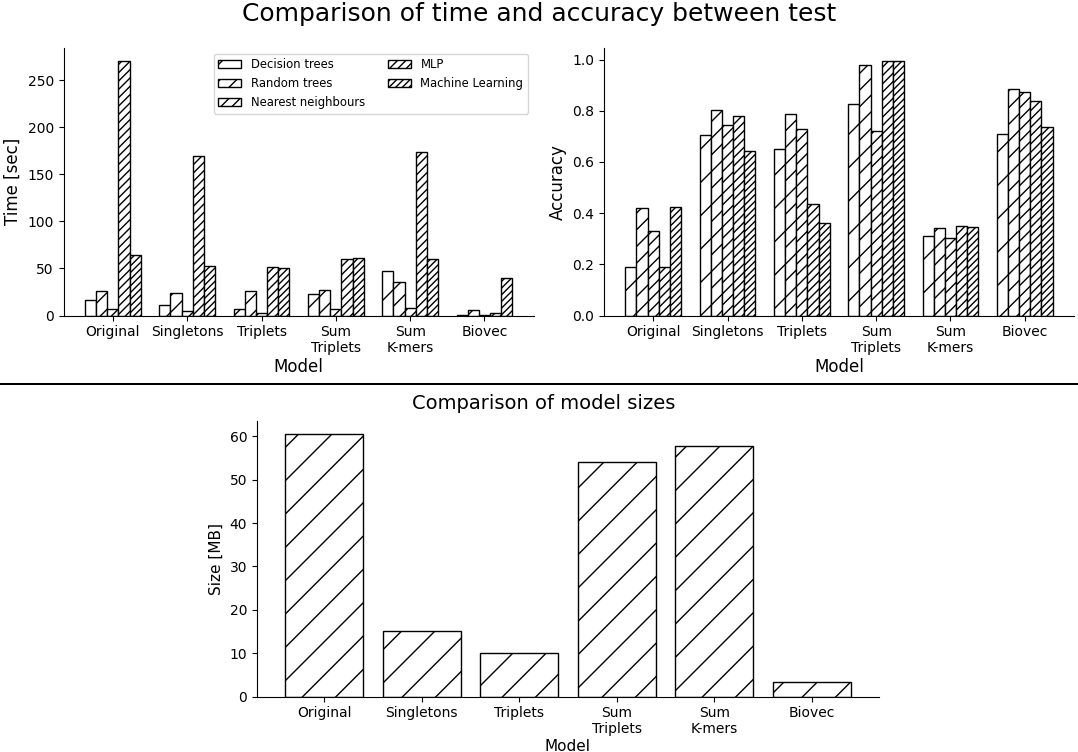
\includegraphics[width=\textwidth]{full_benchmark}
\caption{Test benchmark across all tested datasets, models and comparison of file sizes after encoding. Data preprocessing results in increased test accuracy while significantly reducing the runtime. However, a too strict reduction might lead to loss of information like in the example of ''Sum K-mers''. While speed is closely correlated to the size, the best accuracy was achieved for the ''Sum Triplets'' dataset.}
\end{center}
\end{figure}

As expected, however, not every method yields higher quality classification models. We might speculate the reason behind this is the loss of information. For example, the triplet-encoded sequence was worse than the singleton-encoded one. Similar to sum-vectors. K-mers of size 7 gave unacceptable results compared to 3-mers.

Using BioVec allowed us to reduce the dataset size by over 17 times (from 63,4 MB to 3,6 MB) and speed up training even 120 times (MLP model -- 270,7 sec to 2,25 sec) compared to the original one. In many cases this might be enough to progress with the research. However, researchers, as experts in their fields, should start by analyzing their data first. Early filtering and noise reduction might be crucial for achieving the best results. 

What might be surprising is that BioVec, while crushing the competition with both size and speed, on average, actually gave slightly worse results than the sum of 3-mers. This might suggest that BioVec, while universally applicable, might sometimes be substituted for specific tasks. In this project highest achieved test accuracy reached 99.52\% and 99.24\% for the sum of triplets preprocessing, MLP and Machine Learning models, respectively. 

As for the future of data preprocessing, we should look into more interdisciplinary approaches, as suggested by the BioVec project. Knowledge from the natural language processing field might be essential for further improvement. Pattern searching, motifs, context analyses, relations between fragments -- those topics might allow us to perform wide-range analysis not only for classification but also for more complex, high-level studies of protein structures or topology.

Another result of the project is the provided code. For ease of use, the main workflow is implemented in Jupyter Notebook and is using widgets for the most of the parameters. While default values are identical to those presented in this article, code is provided with an open license allowing modifications and extensions. Furthermore, modular architecture encourages comparing novel models and tweaking hyperparameters of the existing ones to find the best combination for the research problem.


\section*{References}
\begin{footnotesize}
\begin{enumerate}
\item The UniProt Consortium, UniProt: the universal protein knowledgebase in 2021, Nucleic Acids Research, Volume 49, Issue D1, 8 January 2021, Pages D480–D489, \\ https://doi.org/10.1093/nar/gkaa1100
\item Jaina Mistry, Sara Chuguransky, Lowri Williams, Matloob Qureshi, Gustavo A Salazar, Erik L L Sonnhammer, Silvio C E Tosatto, Lisanna Paladin, Shriya Raj, Lorna J Richardson, Robert D Finn, Alex Bateman, Pfam: The protein families database in 2021, Nucleic Acids Research, Volume 49, Issue D1, 8 January 2021, Pages D412–D419, \\ https://doi.org/10.1093/nar/gkaa913
\item Li W, Godzik A. Cd-hit: a fast program for clustering and comparing large sets of protein or nucleotide sequences. Bioinformatics. 2006 Jul 1;22(13):1658-9. doi: 10.1093/bioinformatics/btl158. Epub 2006 May 26. PMID: 16731699.
\item Asgari, Ehsaneddin \& Mofrad, Mohammad. (2015). ProtVec: A Continuous Distributed Representation of Biological Sequences. 
\item Yandell, M., Majoros, W. Genomics and natural language processing. Nat Rev Genet 3, 601–610 (2002). https://doi.org/10.1038/nrg861
\item Mikolov, Tomas et al. “Efficient Estimation of Word Representations in Vector Space.” ICLR (2013).
\item Lee EK. Large-scale optimization-based classification models in medicine and biology. Ann Biomed Eng. 2007 Jun;35(6):1095-109. doi: 10.1007/s10439-007-9317-7. Epub 2007 May 15. PMID: 17503186.
\item Radzi SFM, Karim MKA, Saripan MI, Rahman MAA, Isa INC, Ibahim MJ. Hyperparameter Tuning and Pipeline Optimization via Grid Search Method and Tree-Based AutoML in Breast Cancer Prediction. J Pers Med. 2021;11(10):978. Published 2021 Sep 29. doi:10.3390/jpm11100978
\item Abraham A, Pedregosa F, Eickenberg M, et al. Machine learning for neuroimaging with scikit-learn. Front Neuroinform. 2014;8:14. Published 2014 Feb 21. doi:10.3389/fninf.2014.00014
\end{enumerate}
\end{footnotesize}
\newpage

\section*{Additional information}
\subsubsection*{Workflow}
Result workflow can be accessed on Github: \\ https://github.com/exsto1/Protein-sequence-preprocessing-benchmark-for-classification-task-Maciej-Sikora

All required information about setup and usage is described in the Readme file.

\subsubsection*{Grid Search parameters}
\begin{center}
\begin{tabular}{ | l | l | l |} 
\hline
Model & Parameters & N. of iterations\\ 
\hline
\hline
Decision Trees & Max Depth: [10, 20, 30, 40, 50, 60, 70, 80, 90, 100] & 20\\
\hline
Random Trees & Max Depth: [10, 20, 30, 40, 50] & 30\\ 
 & Max Features: [10, 15, 20] & \\ 
\hline
Nearest Neighbours & Weights: [Uniform, Distance] & 4 \\ 
\hline
MLP & Hidden Layer Sizes: [32, 64, 128] & 6\\ 
\hline
Machine Learning & Layers: [2, 3] & 36\\
 & Layer sizes: [16, 64, 512] & \\
 & Tested all possible combinations of layer sizes given depth & \\
\hline
\end{tabular}
\end{center}

\end{document}